% Provide your results:
%       clearly
\begin{frame}
\frametitle{Validation of Scaling and Superposition}
\footnotesize{

\begin{figure}[htp!]
\begin{center}
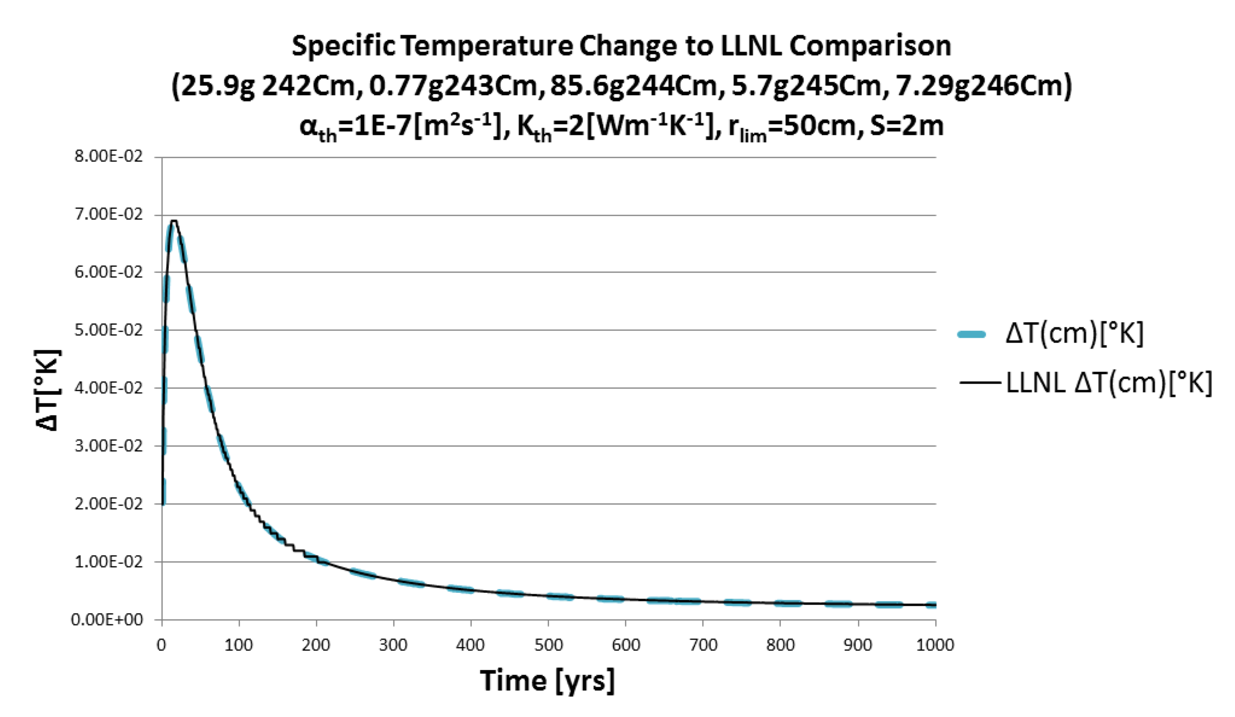
\includegraphics[width=\columnwidth]{./cyder/thermal_models/CmValidation.eps}
\end{center}
\caption{This comparison of \gls{STC} calculated thermal response from $Cm$ 
inventory per MTHM in 51GWd UOX PWR fuel compares favorably with results 
from the analytical model from LLNL. This example, with no neglected nuclides, 
has an average error of 1.1\% and a maximum error of 4.4\%.
} 
\label{fig:CmValidation}
\end{figure}
}
\end{frame}

\begin{frame}[ctb!]
\frametitle{Boundedness of Capacity Estimation}
Inaccuracies from neglected low heat contributing nuclides are bounded. 
Specifically, since the highest heat contributing nuclides are accounted for, 
most innacuracies will arise from lower heat contributing nuclides. The maximum 
underestimate by this model is therefore less than the difference that would 
arise if all of the unnaccounted for nuclides had the heat generation of the 
coolest of the high-heat generating nuclides.
\end{frame}
